\documentclass[a4j,twocolumn,10pt]{jarticle}
\usepackage{dia2022}
\usepackage{color}

\makeatletter
%%%タイトル調整
\setcounter{totalnumber}{3}
\def\id#1{\def\@id{#1}}
\def\@maketitle{%
\vspace{-4.3em}
\begin{center}%
{\@title \par}% タイトル
{\@author}% 著者
\end{center}%
%\par\vskip 1.5em
}
\makeatother

\title{
\vspace{15mm}
\Large{
\textbf{\leftline{【若手研究奨励賞候補:はい/いいえ】(該当する方を残して下さい)}}\\
\textbf{DIA2022動的画像処理実利用化ワークショップ(講演題目をお書き下さい)}} %%%%%%論文タイトルを記入
}

\author{
\vspace{1.5em}
\large{○平成太郎 $\dagger$,} %%%%著者1->著者名1に書き換え,【重要】講演者に○を付けてください!
\large{ウィリアム・テイラー $\ddagger$}\\                 %%%%著者2->著者名2に書き換え
\vspace{1em}
\large{{\rm ○ Taro HEISEI $\dagger$\ }             %%%%Author1->著者名1ローマ字に書き換え
{\rm and\ }
{\rm William TAYLOR $\ddagger$} }\\     %%%%Author2->著者名2ローマ字に書き換え
\vspace{0.5em}
\large{$\dagger$:画像科学技術大学理工学部,}     %%%%所属1->著者1の所属に書き換え
{\rm taro@image.eng.u-pc.ac.jp} \\                    %%%%著者1のメールアドレス
\large{$\ddagger$:Soho Corporation,}    %%%%所属2->著者2の所属に書き換え
{\rm taylor@soho.com }\\                     %%%%著者2のメールアドレス
}
\date{} %日付を表示しない
\pagestyle{empty}

\setstretch{1.1} %%%行間隔調整用:適宜調整してください.
%\pagestyle{empty}
\begin{document}
%---タイトル---
\twocolumn[
\maketitle
\thispagestyle{empty} %maketitleをいじっている関係でここでページ番号を消去
\vspace{-2em}
\begin{abstract}
 \noindent{}<要約>これは,【提出物1】申込み用講演概要原稿(およそ2ページ)の様式です.\\
 <キーワード>○○○,○○○,○○○,○○○,○○○ (キーワードを3~5語お書き下さい)
\vspace{2.5em}
\end{abstract}]
\vspace{1em}

%--- 本文開始 ---
\section{若手研究奨励賞について}
2022年3月3日時点で35歳以下の発表者は,若手研究奨励賞の候補となります.
候補者は,タイトル上にある選択肢の「はい」を残してください(いいえを削除してください).
そうでない方は,「いいえ」を残してください(「はい」を削除してください).

\section{講演申込み手順}

\subsection{OpenConfでID番号の取得}

DIA2022のホームページ(http://www.tc-iaip.org/dia/2022/)にある「講演申込」からか,次のURL先(https://www.tc-iaip.org/dia/2022/openconf/)よりOpenConfへアクセスし,「サブミッションの作成」で必要事項を入力してID番号を発行してください.

\subsection{申込み用講演概要原稿の作成}

\underline{【提出物1】申込み用講演概要原稿}は,A4用紙\textcolor{red}{2ページ程度}で発表内容を分かりやすく,発表内容が十分理解できるように記述して下さい.図,グラフ等を用いても結構です.

\subsection{申込み用講演概要原稿のアップロード}

OpenConfへアクセスし,発行したID番号と自分で設定したパスワードを使用して「ファイルのアップロード」より\underline{【提出物1】申込み用講演概要原稿}をアップロードして下さい.アップロードするファイルはPDF形式で,\textcolor{red}{5MB以下}として下さい.

\fbox{\textcolor{red}{提出期限は, 2021年12月3日(金)です!}}

\subsection{講演形式}

講演形式(インタラクティブ/オーラルセッション)についてはプログラム委員会で決定します.ご希望に添えない場合もございます.予めご了承下さい.1月中旬までにご連絡いたします.


\section{原稿の構成と体裁}

\subsection{用紙の設定}

用紙はA4,余白は上30mm,下30mm,左20mm,右20mmです.

\subsection{原稿の構成}

原稿は,表題欄,著者欄,要約欄,本文欄,参考文献欄などから構成されています.

\subsection{表題欄の体裁}

表題欄は上から30mm,1段組でセンタリングとします.文字は14ポイント,改行は21ポイント,書体はゴシック体の太文字を使用してください.副題は,“-”(ハイフン)ではさむなど,適宜処理してください.

\subsection{著者欄の体裁}

著者欄は上から50mm,1段組でセンタリング.最初に著者名(+連名者),次の行に所属をお書きください.文字は12ポイント,改行は18ポイント.表題欄との間隔は10mm程度にしてください.

\subsection{要約欄の体裁}

要約欄は1段組で均等配置とします.文字は10ポイント,改行は15ポイントです.先頭は全角1文字程度下げてください.著者欄との間隔が10mm程度となるように調整してください.

\renewcommand{\arraystretch}{1.5}
\begin{table}[h]
\caption{原稿の長さ}
\vspace{-5mm} 
\label{tbl}

\begin{center}
\small
\begin{tabular}{p{3.5cm}|p{3.5cm}} \hline
(1)申込み用講演概要原稿 & 2ページ(カラー可) \\ \hline
\end{tabular}
\end{center}
\end{table}


\subsection{本文の体裁}

本文は2段組で均等配置とします.章タイトルは字下げせず,1. 2. 3. …とし,文字は12ポイントとして下さい.節は2.1, 2.2, 2.3…とし,段落開始時には1字下げてください.文字の大きさは10ポイント,改行幅は15ポイントです.文字数は全角23文字/行/カラムです. 2頁以降は48行/カラムです.

\subsection{図・表,写真の体裁}

鮮明なものをご用意ください.また,図・表内の文字は小さくなりすぎないよう注意してください.

\renewcommand{\arraystretch}{1.0}
\begin{figure}[h]
\centering
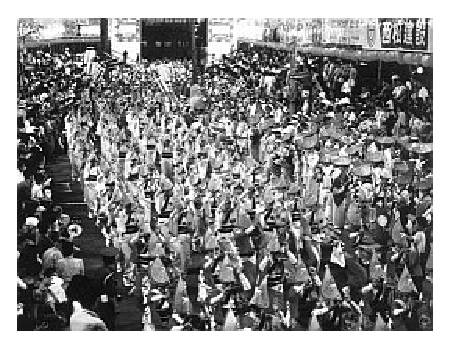
\includegraphics[width=40mm]{awaodori.eps}
\caption{阿波踊り}
\label{fig:graph3}
\end{figure}

漢字の場合は8ポイントが限界です.


\section{お問い合わせ先}

何か問題が生じた場合には,OpenConfの「お問い合わせ」からか,以下の事務局にご相談下さい.

\hspace{-5mm}
\fbox{
\renewcommand{\arraystretch}{1.0}
\small
\begin{tabular}{l}
アドコム・メディア(株)内 \\
画像応用技術専門委員会事務局 「DIA2022」係 \\
 〒169-0073 新宿区百人町2-21-27 \\
 TEL:03-3367-0571 \\
 e-mail: iaip@adcom-media.co.jp \\
\end{tabular}
}

\begin{thebibliography}{9}
\bibitem {1} 寺田賢治:“動的画像処理”,動的画像処理実利用化ワークショップ2018講演論文集,Vol.1, No23, pp.456-789 (2018)
\bibitem {2} 寺田賢治:“密集する不定形状な泡の計数”,外観検査アルゴリズムコンテスト,Vol.9, No.8, pp.765-4321 (2015)
\end{thebibliography}

\end{document}
